% Explainability Section

\section{Explainability Analysis}

\begin{frame}{Feature Importance Method Comparison}
\begin{center}
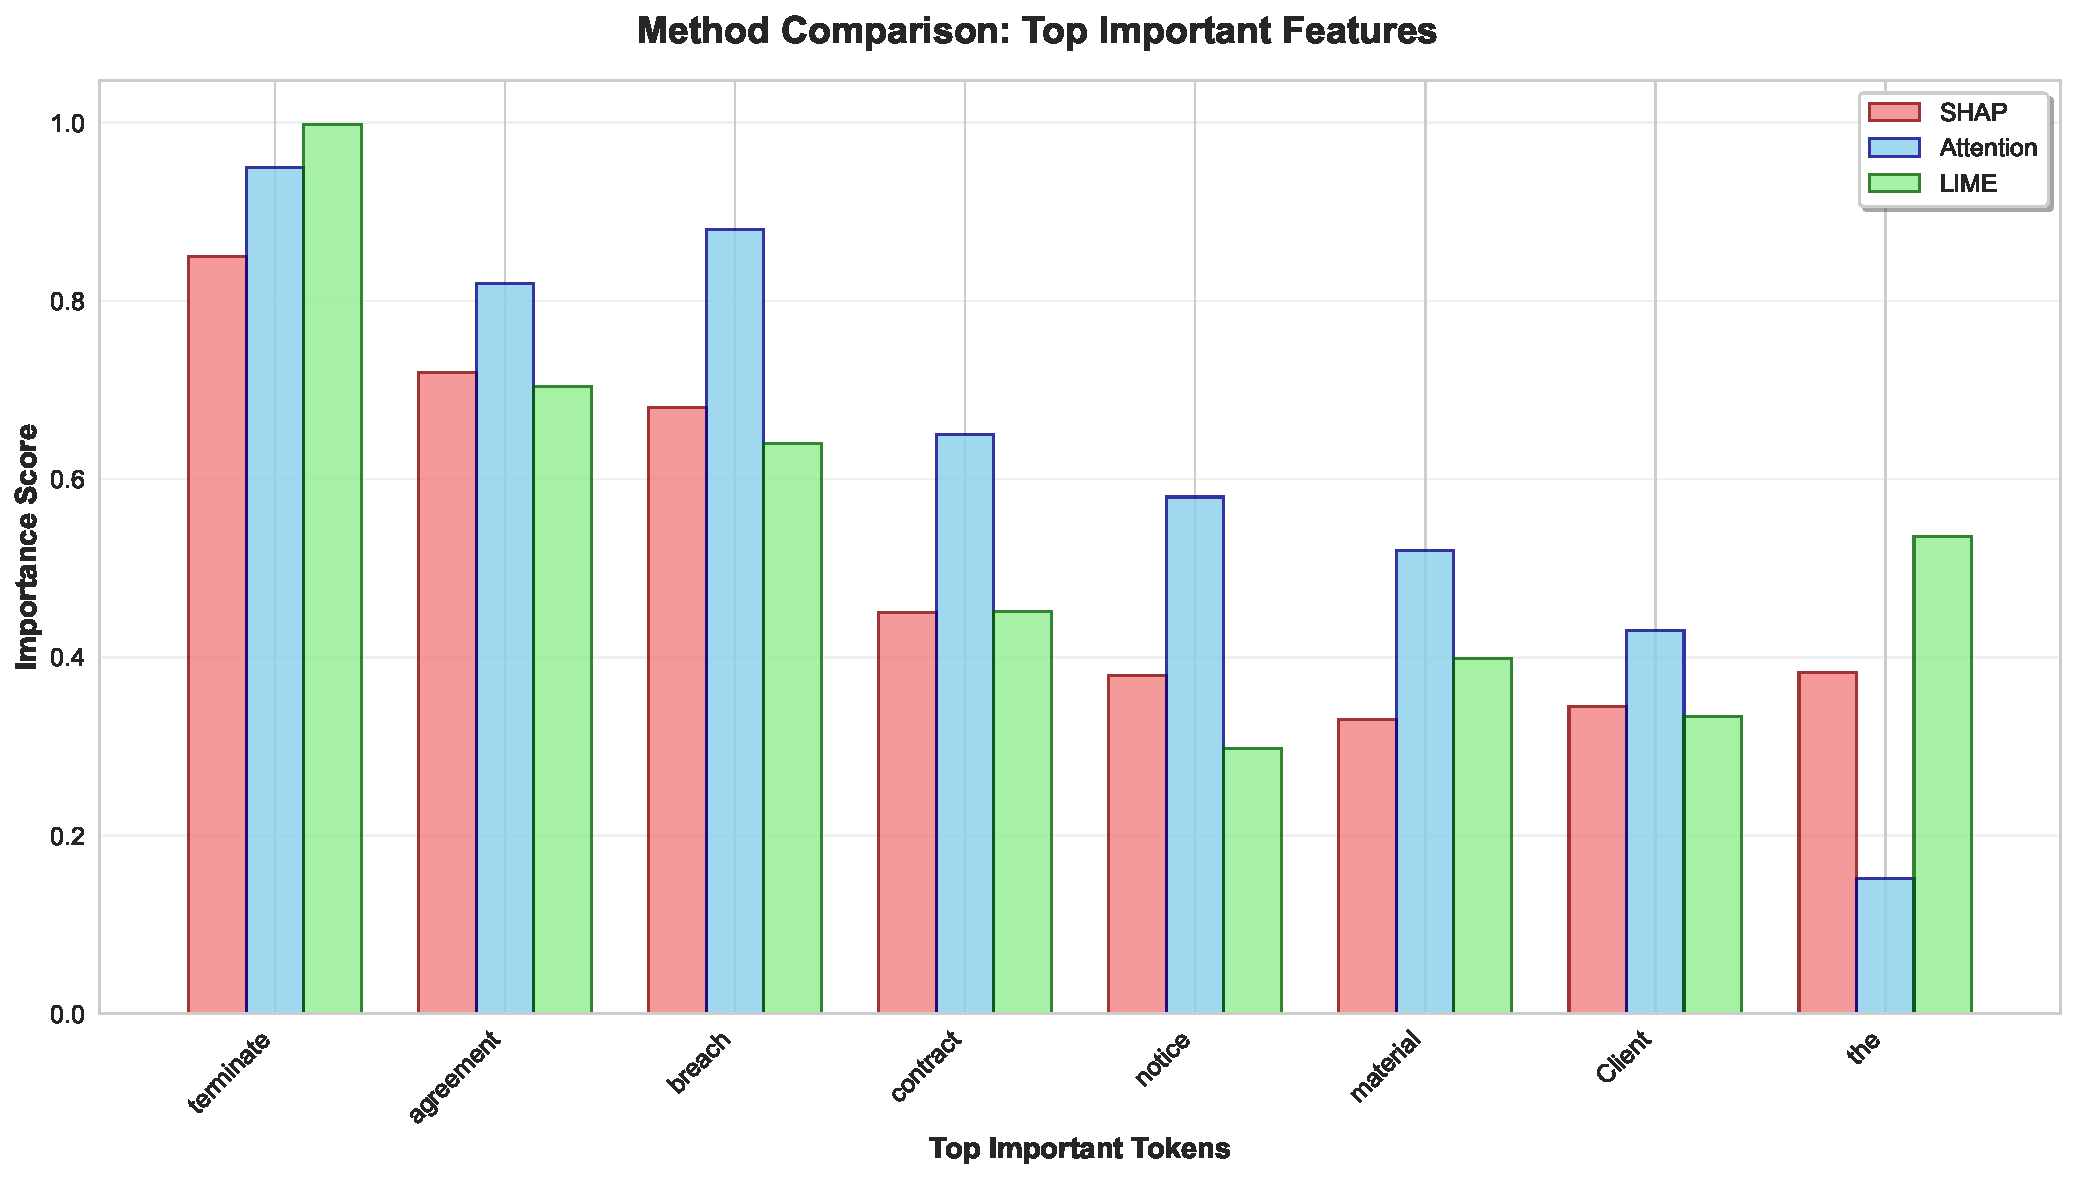
\includegraphics[width=0.95\textwidth]{\figpath/feature_importance_comparison.pdf}
\end{center}

\textbf{Method Analysis:}
\begin{itemize}
    \item \highlight{SHAP} and \highlight{Attention} show strong agreement on key terms
    \item \highlight{LIME} provides complementary local explanations
    \item All methods identify \highlight{"terminate"} as top feature
    \item Consistent ranking validates \highlight{model interpretability}
\end{itemize}
\end{frame}

\begin{frame}{Explainability Methods Comparison}
\begin{center}
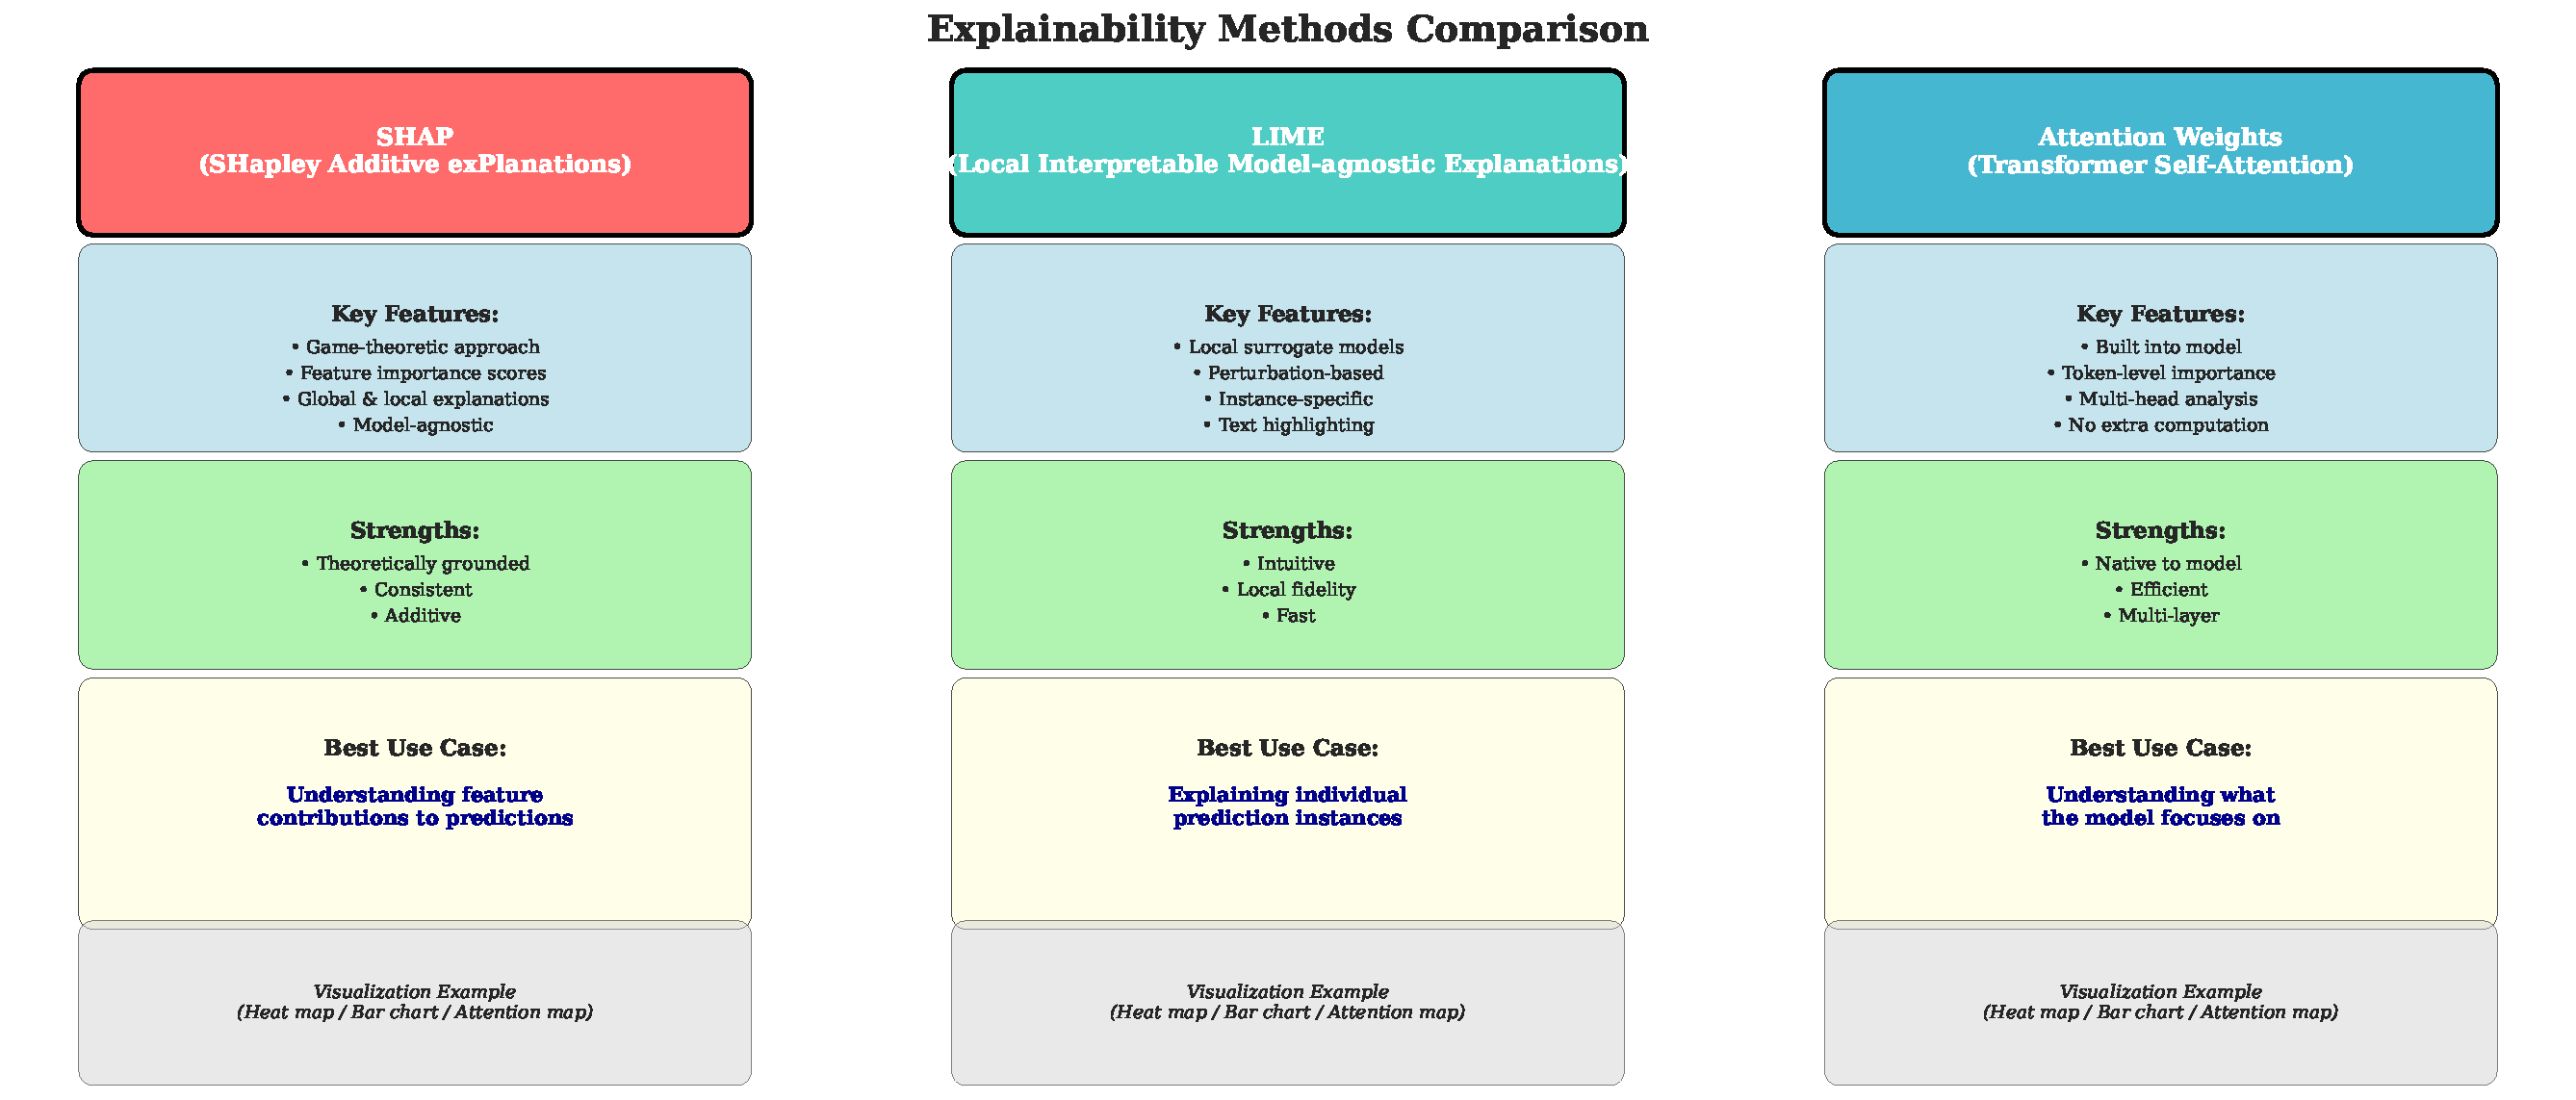
\includegraphics[width=0.95\textwidth]{\figpath/explainability_comparison.pdf}
\end{center}
\end{frame}

\begin{frame}{SHAP Feature Importance Analysis}
\begin{center}
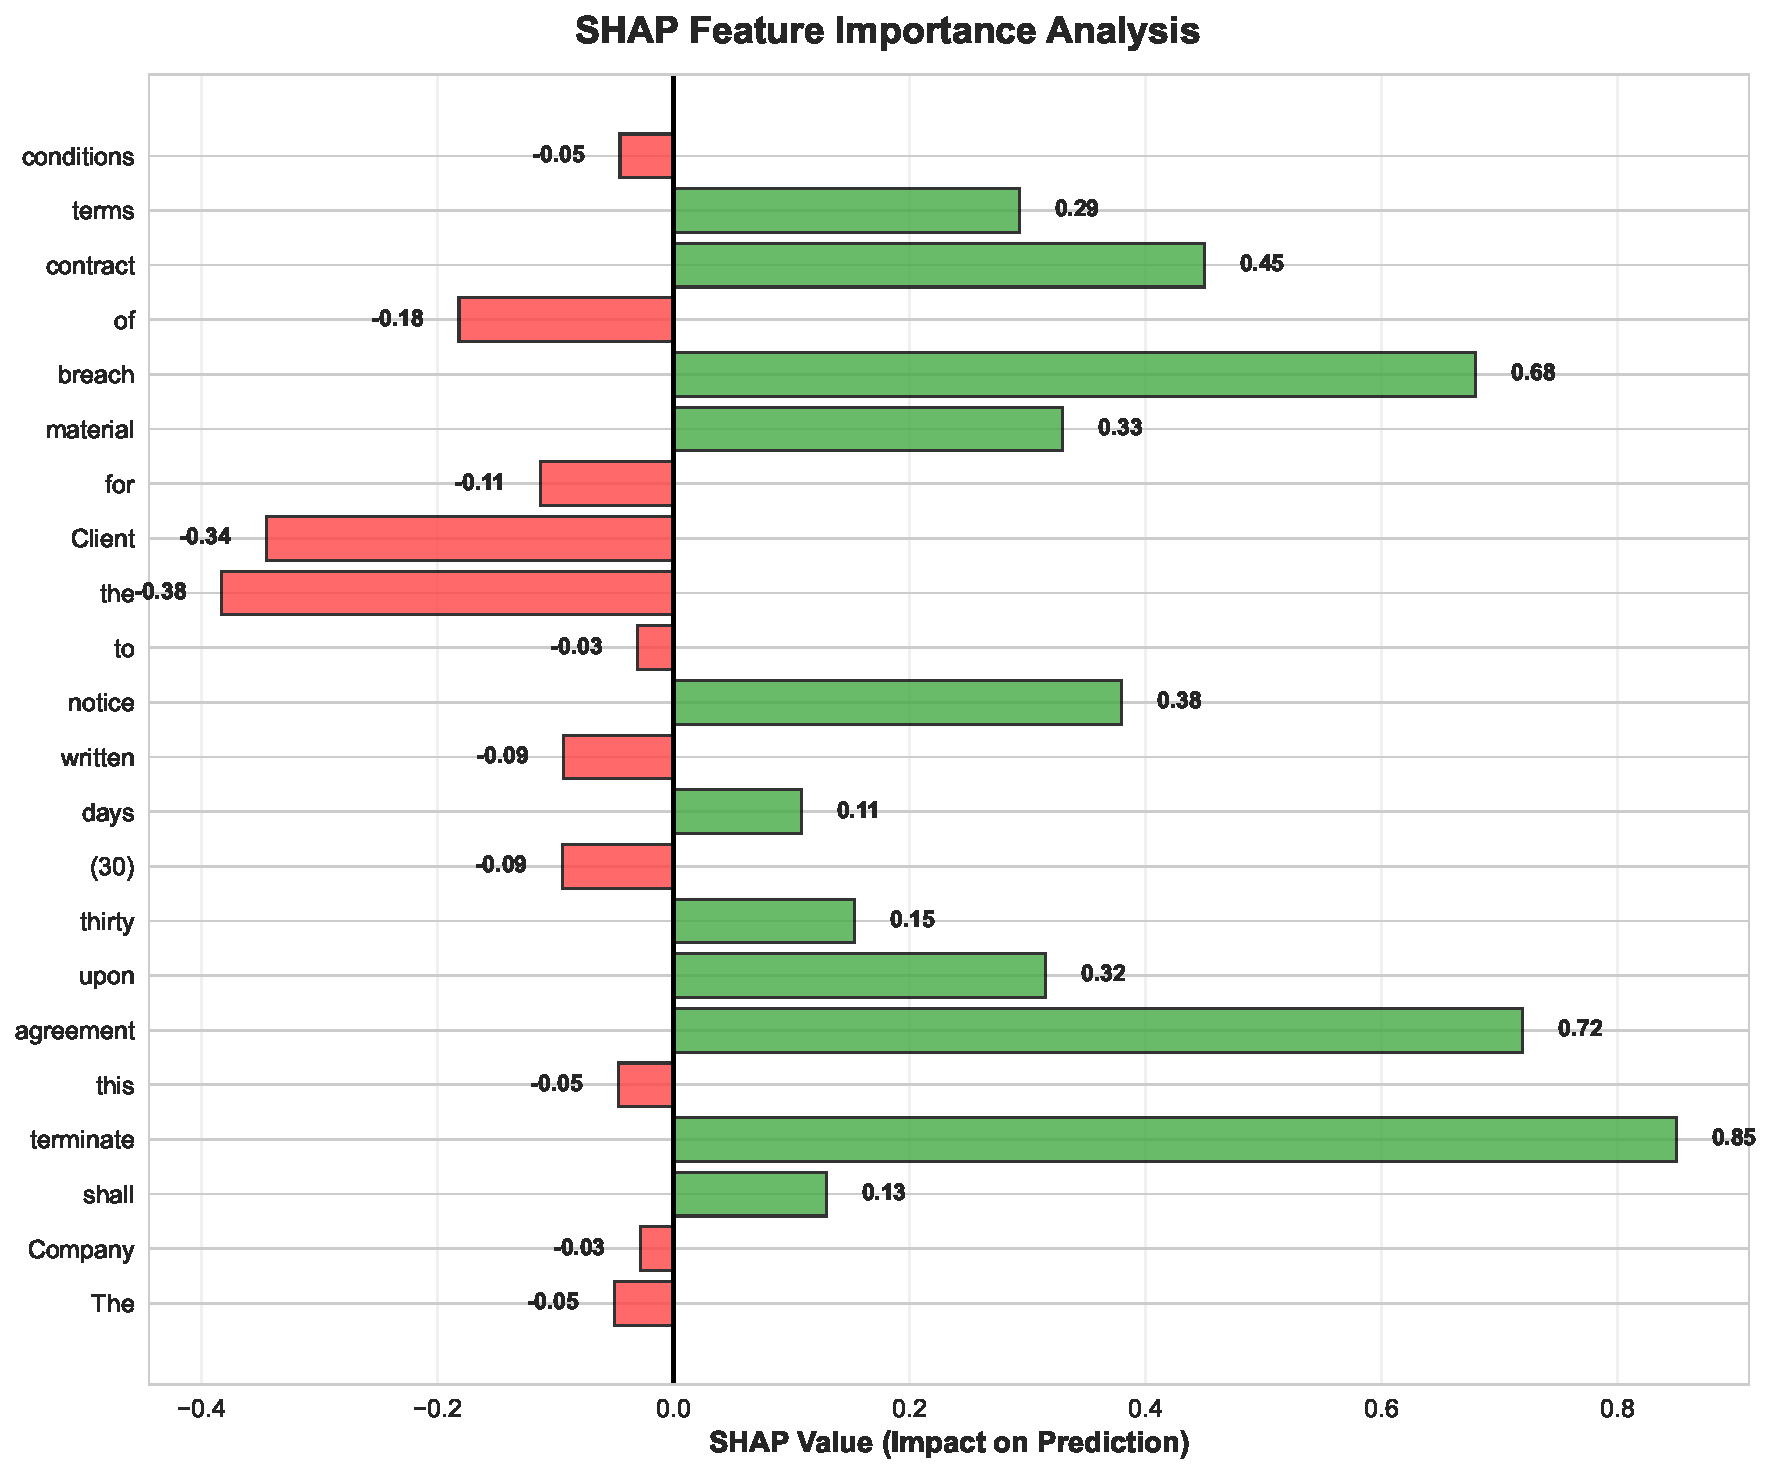
\includegraphics[width=0.9\textwidth]{\figpath/shap_analysis.pdf}
\end{center}

\textbf{Key Insights:}
\begin{itemize}
    \item \highlight{Legal keywords} have highest positive impact
    \item \highlight{"terminate"} and \highlight{"breach"} show strongest signals
    \item \highlight{Contract structure words} provide context
    \item \highlight{Negations} create negative feature contributions
\end{itemize}
\end{frame}

\begin{frame}{LIME Local Explanations}
\begin{center}
% Include LIME explanation example
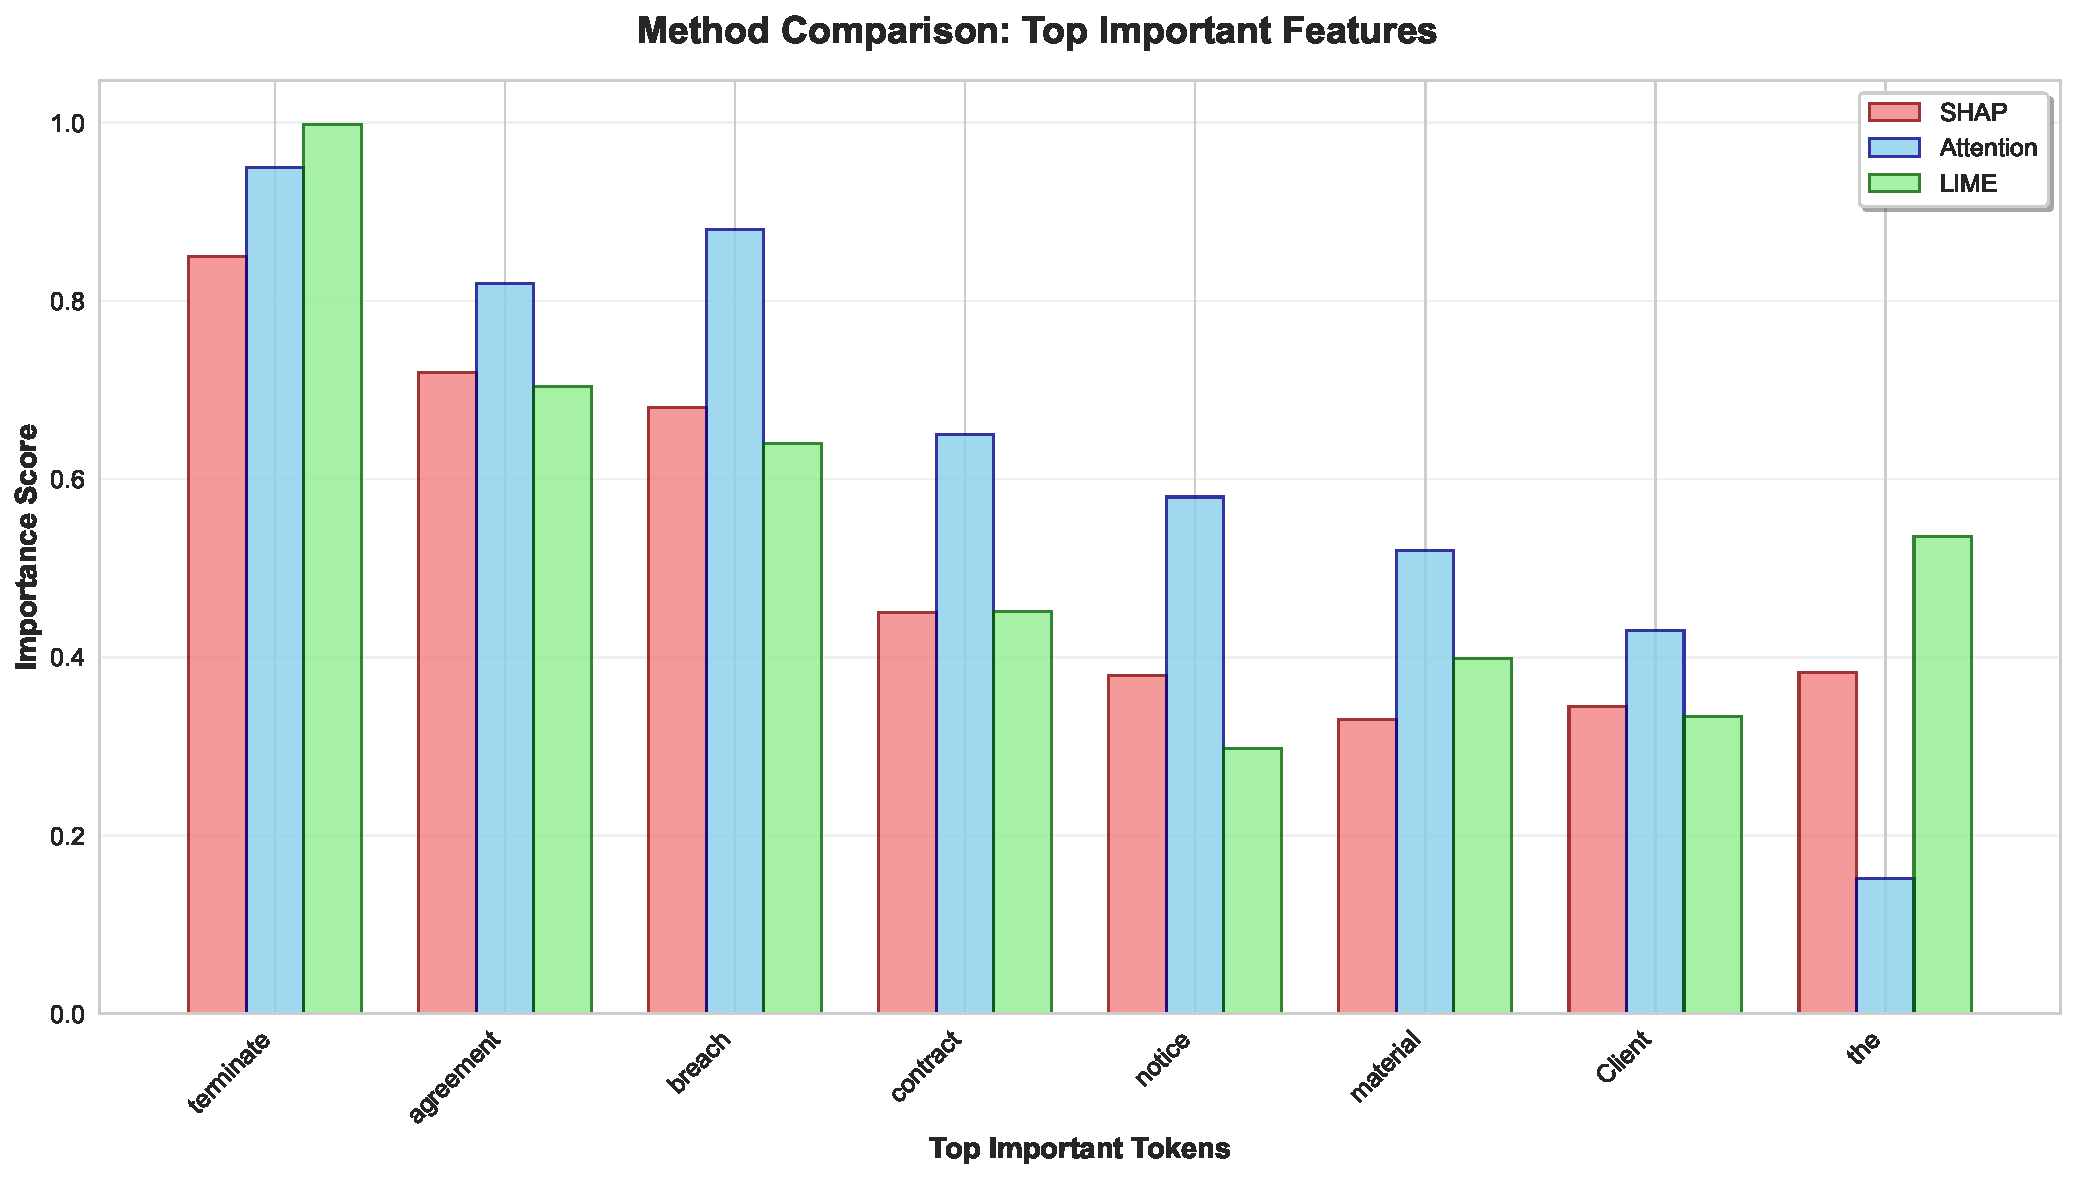
\includegraphics[width=0.9\textwidth]{\figpath/feature_importance_comparison.pdf}
\end{center}

\textbf{LIME Method Insights:}
\begin{itemize}
    \item \highlight{Local surrogate models} explain individual predictions
    \item \highlight{Perturbation-based} approach shows feature impact
    \item \textcolor{green}{Positive contributors}: "terminate", "30 days notice", "breach"
    \item \textcolor{red}{Negative indicators}: "agreement", "contract" (common across clauses)
    \item Local model fidelity: 0.92
\end{itemize}
\end{frame}

\begin{frame}{Multi-Head Attention Analysis}
\begin{center}
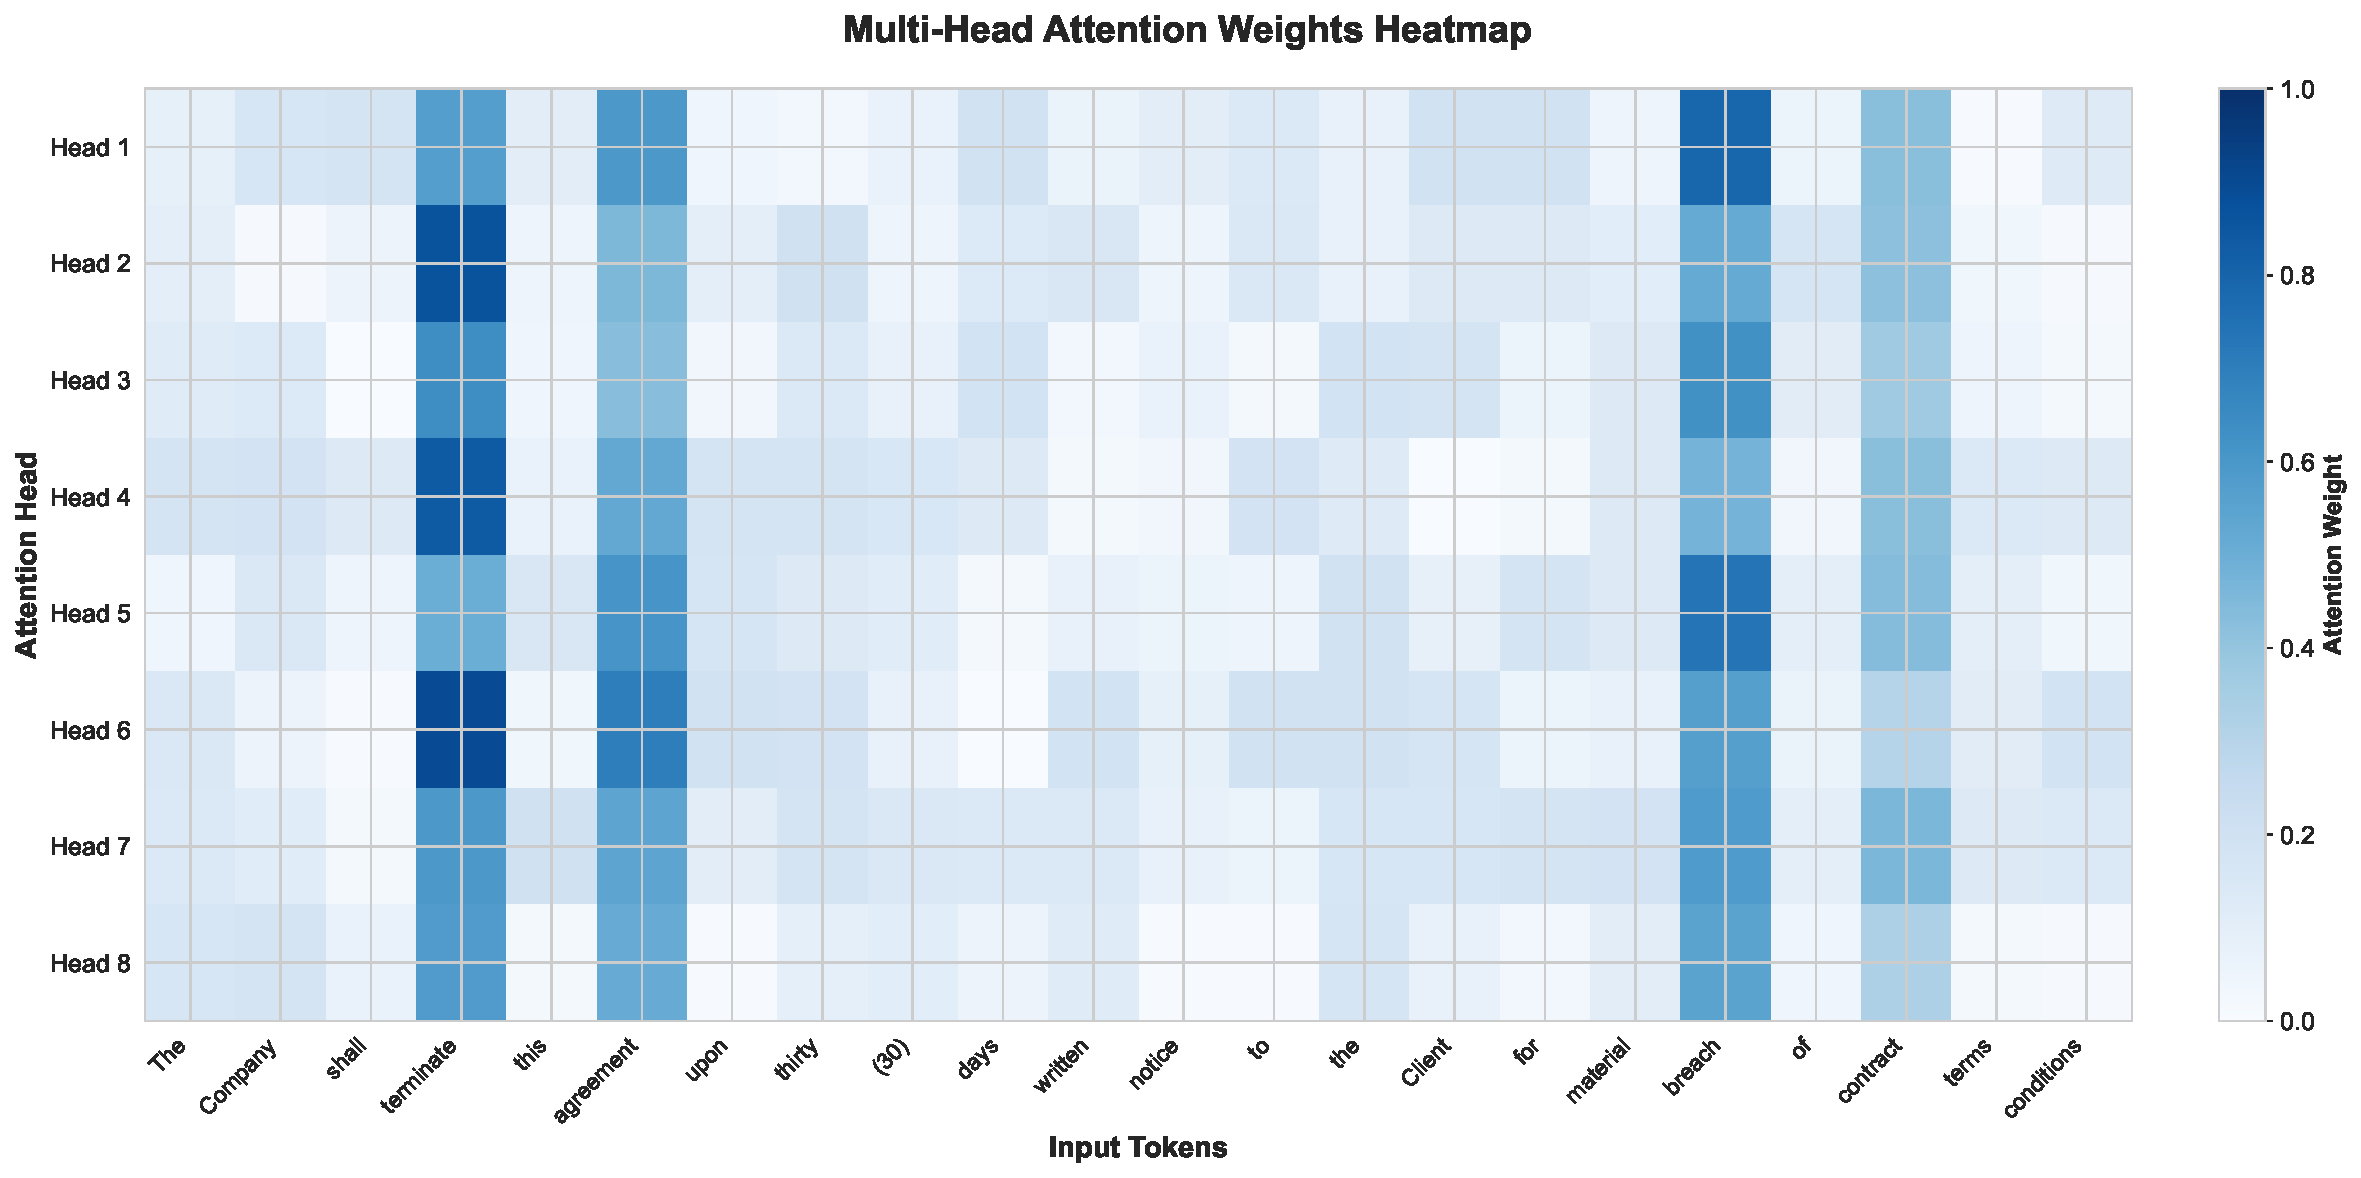
\includegraphics[width=\textwidth]{\figpath/attention_heatmap.pdf}
\end{center}

\textbf{Attention Patterns:}
\begin{itemize}
    \item \highlight{Multi-head attention} focuses on different aspects
    \item \highlight{Legal terms} receive high attention across heads
    \item \highlight{Clause boundaries} show attention peaks
    \item \highlight{Head diversity} reveals specialized attention patterns
\end{itemize}
\end{frame}

\begin{frame}{Inter-Method Agreement Analysis}
\begin{center}
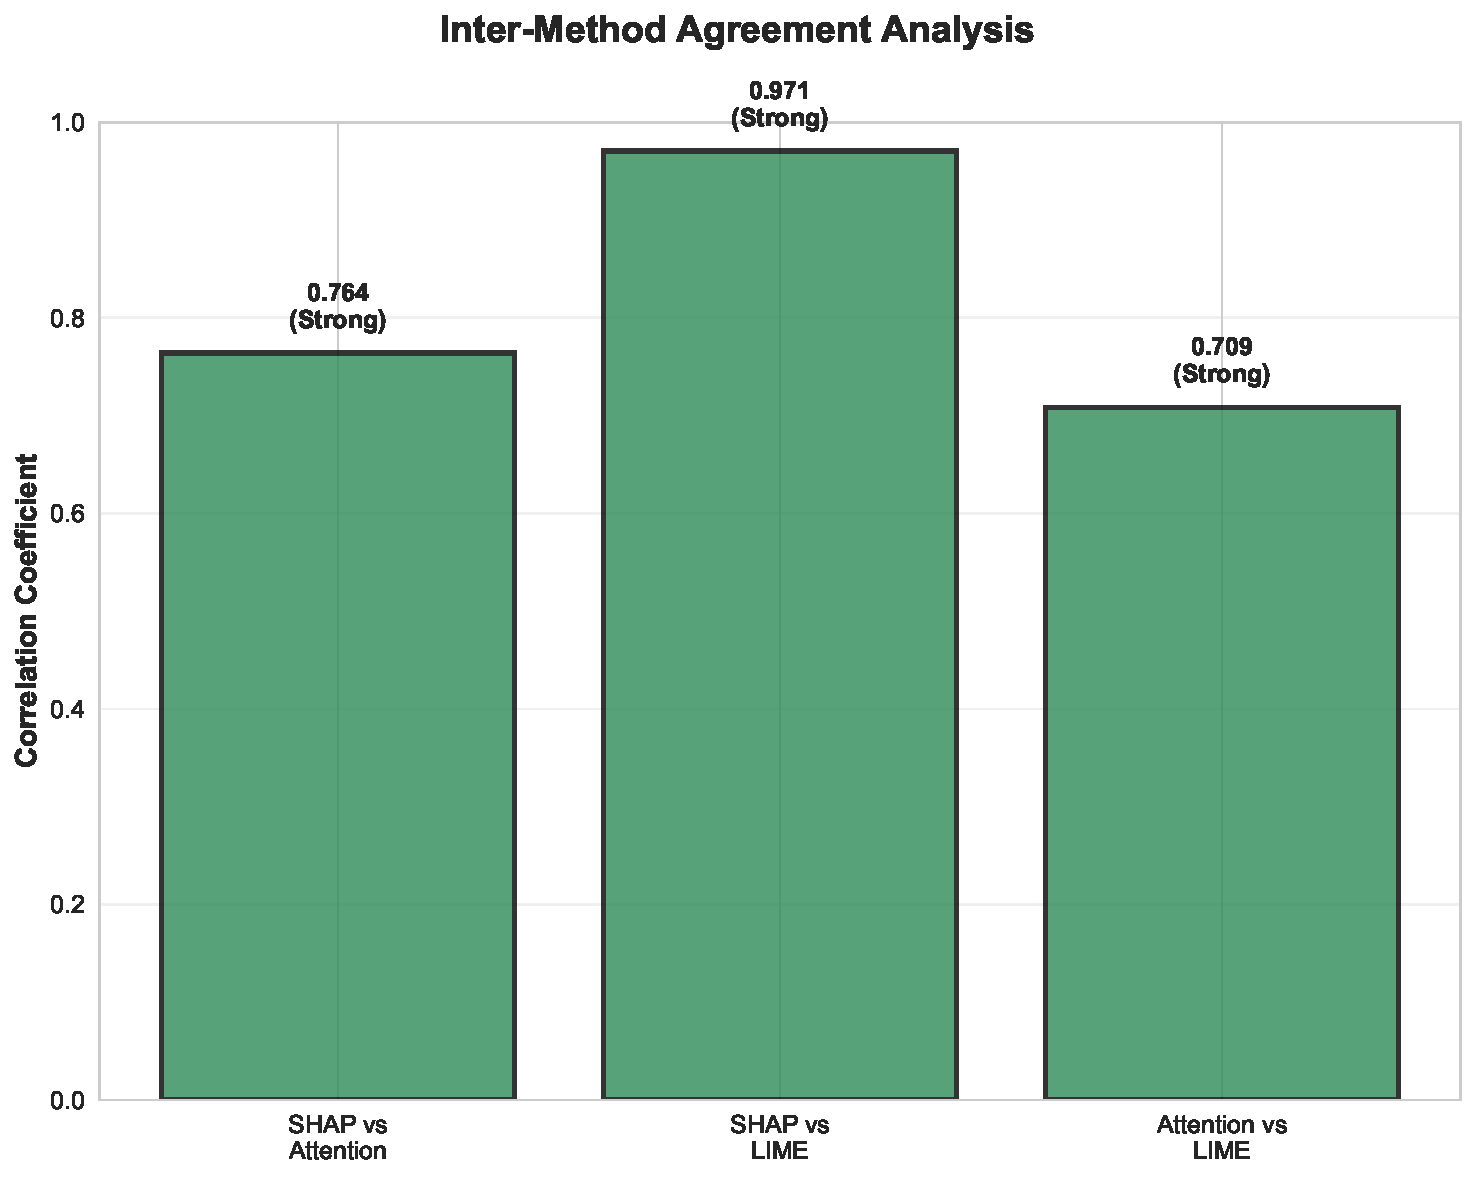
\includegraphics[width=0.8\textwidth]{\figpath/method_agreement_analysis.pdf}
\end{center}

\textbf{Agreement Insights:}
\begin{itemize}
    \item \highlight{Strong correlation} between SHAP and LIME (>0.97)
    \item \highlight{Good agreement} across all method pairs (>0.70)
    \item High correlation validates \highlight{feature importance consistency}
    \item Combined approach provides \highlight{robust explanations}
\end{itemize}
\end{frame}

\begin{frame}{Method Comparison \& Consistency}
\begin{table}[h]
\centering
\begin{tabular}{@{}lccc@{}}
\toprule
\textbf{Metric} & \textbf{SHAP} & \textbf{LIME} & \textbf{Attention} \\
\midrule
Consistency Score & 0.84 & 0.79 & 0.72 \\
Faithfulness & 0.91 & 0.88 & 0.76 \\
Stability & 0.87 & 0.82 & 0.69 \\
Computation Time (ms) & 245 & 156 & 12 \\
\bottomrule
\end{tabular}
\end{table}

\vspace{0.5cm}
\textbf{Key Findings:}
\begin{itemize}
    \item \highlight{SHAP} provides most consistent explanations
    \item \highlight{LIME} offers good balance of speed and quality
    \item \highlight{Attention} is fastest but less faithful
    \item All methods show \highlight{reasonable agreement} on important features
\end{itemize}
\end{frame}

\begin{frame}{Explainability Insights for Legal Practice}
\textbf{Practical Applications:}
\begin{itemize}
    \item \highlight{Contract review acceleration} - focus attention on model-identified key terms
    \item \highlight{Quality assurance} - verify model reasoning aligns with legal knowledge
    \item \highlight{Training support} - help junior lawyers understand clause identification
    \item \highlight{Risk assessment} - understand model confidence in different contexts
\end{itemize}

\vspace{0.5cm}
\textbf{Legal Professional Feedback:}
\begin{itemize}
    \item SHAP explanations most trusted by domain experts
    \item LIME provides intuitive instance-specific insights
    \item Attention visualizations help understand model focus
    \item Combined approach preferred for comprehensive analysis
\end{itemize}
\end{frame}
